%\section{\textcolor{MidnightBlue}{Grundlagen und psychologische Ansätze zur Gestaltung nutzerfreundlicher und moderner Oberflächen in Bezug zur Erstellung von Dashboards}}
\section{\textcolor{Salmon}{Grundlagen und psychologische Ansätze zur Gestaltung nutzerfreundlicher und moderner Dash\-boards}}
\label{ch:SdF:UI}

\textcolor{red}{TODO: Einleitungsabsatz}\\
Human Machine Interface\\
--> Teil der Maschine, dieInformationen an den Menschen übermittelt\\
--> womit der Mensch die Maschine bedienen kann\\

\noindent
kognitive Ergonomie\\
--> ist ein Fachgebiet, dass sich in besonderer Weise mit der Interaktion von Mensch und Maschine befassen sollte\\
--> Ergonomie: das gute Produkt steht im Vordergrund\\
--> Ingenieurspsychologie: stärker konzentriert auf den Menschen und das Verstehen der Prozesse

\cite{Vollrath:2015:Taschenbuch}

% ******* ISO *********************
\subsection{ISO-Normenreihe 9241 zur Gebrauchstauglichkeit und Ergonomie interaktiver Systeme}
\label{ch:SdF:UI:ISO}

Die Normen unter der DIN EN ISO 9241 aus dem Jahr 2020 geben Vorgaben und Empfehlungen zur Gestaltung interaktiver Systeme.
\autoref{fig:iso-uebersicht} stellt den Zusammenhang der Hauptquellen für Empfehlungen zur Benutzer-System-Interaktion dar. Es sind die Parts 11, 110, 112 und weitere zu erkennen. Die DIN EN ISO 9241-11 definiert den Begriff Usability, %(dt. Gebrauchstauglichkeit)
währenddessen Part 110 und 112 Prinzipien und Grundsätze mitgeben, um die Usability eines Systems gewährleisten zu können.

\begin{figure}[H]
    \centering
    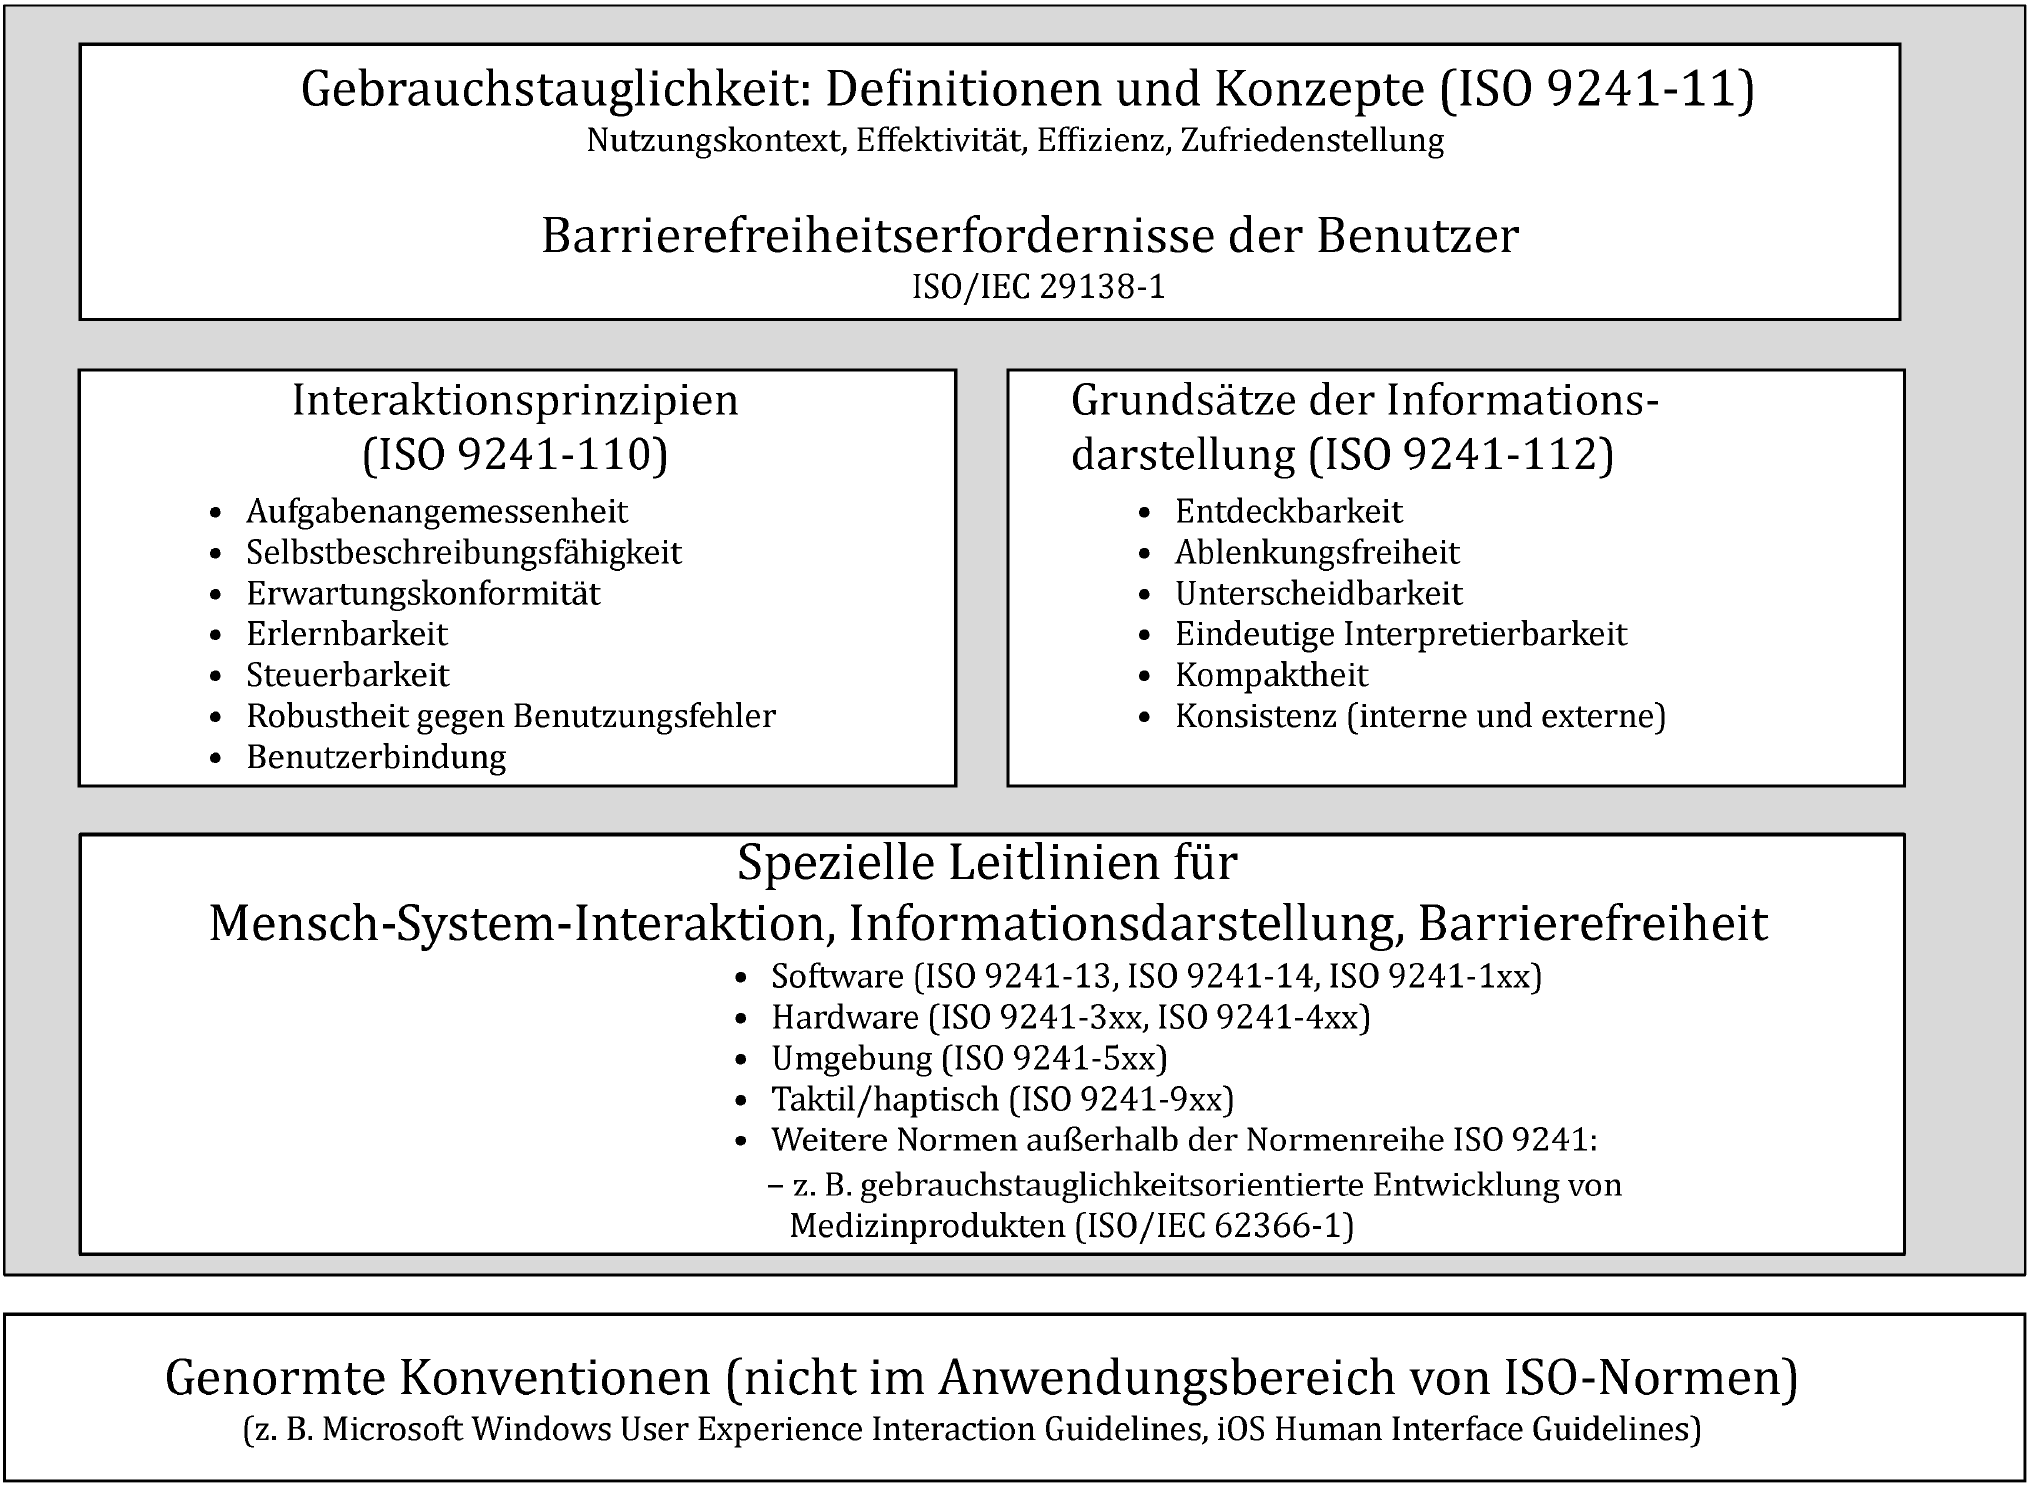
\includegraphics[width=1\linewidth]{chapters/02_Stand_der_Forschung/ISO-Normen_Uebersicht.PNG}
    %\caption{Überblick und Zusammenspiel der ISO-Normen mit Fokus auf die Usability von interaktiven Systemen \cite{DIN_EN_ISO_9241-110}}
    \caption{\glqq Beziehung zwischen den Hauptquellen für Empfehlungen zur Benutzer-System-Interaktion\grqq{} \cite{DIN_EN_ISO_9241-110} mit Fokus auf die Usability}   % S. 16
    \label{fig:iso-uebersicht}
\end{figure}

\noindent
%In den folgenden Kapiteln werden die Inhalte der DIN EN ISO 9241-110 Interaktionsprinzipien (ISO 9241-110:2020) \cite{DIN_EN_ISO_9241-110} mit Fokus zur Anwendung auf Dashboards zusammengefasst.
Die DIN-Normen sind in diesem Fall die nationale Umsetzung der internationalen ISO-Normen und werden nachfolgend synonym mit ‚ISO‘ referenziert.

\subsection{Definition Usability nach ISO 9241-11}
\label{ch:SdF:UI:sec:Usability}
Der Begriff der Usability (dt. Gebrauchstauglichkeit) beschreibt die Qualität eines Systems oder einer Oberfläche in Bezug auf dessen Einfachheit und Nutzbarkeit. Diese wird gemessen in den Dimensionen der Effektivität, Effizienz und der Zufriedenheit der Nutzer.

Die Effektivität beschreibt die funktionelle Eignung eines Systems. Das heißt, dass der Nutzer seine Aufgaben vollständig und korrekt mithilfe dieses Systems durchführen kann. Die Effizienz misst sich in Form von Zeit, um eine Aufgabe vollständig und richtig zu erfüllen, und der Rate, wie viele Fehler auf dem Weg dorthin gemacht werden. Die Zufriedenheit oder auch Akzeptanz (en. Satisfaction) \cite{Vollrath:2015:Taschenbuch} der Nutzer ist nicht in metrischen Kenngrößen zu erfassen. Es kann ein Zufriedenheitsspektrum auf Grundlage von zum Beispiel Fragebögen (s. \autoref{ch:SdF:UI:sec:ISO-Fragebogen}) oder der Verhaltensanalyse während eines Testszenarios festgestellt werden. [Zusammenfassung nach \cite{DIN_EN_ISO_9241-110}]

% ******************************************************************
\subsection{Definition User-Experience und Abgrenzung von Usability}
\label{ch:SdF:UI:sec:Usability_vs_User_Experience}
Neben der Usability steht die User-Experience (UX, dt. Nutzererfahrung oder -erlebnis). Dessen Inhalte leicht verwechselt werden. Die User-Experience wird in Part 210 der ISO 9241 definiert als \glqq Wahrnehmungen und Reaktionen einer Person, die aus der tatsächlichen und/oder der erwarteten Benutzung eines Produktes, eines Systems oder einer Dienstleitung resultieren.\grqq{} \cite[S. 7]{DIN_EN_ISO_9241-210:2011}

Während bei der Usability die schnelle, fehlerfreie und angenehme Bedienung eines Systems im Vordergrund stehen, wird die User-Experience zusätzlich mit Spaß, Vergnügen und positivem Erleben verbunden \cite{Vollrath:2015:Taschenbuch}.

Da die Gebrauchstauglichkeit (UE) ein Part des Nutzererlebnisses (UX) ist ($UX \varsubsetneq UE$) \cite{usability_vs_experience:2018} wird diese nicht in \autoref{fig:iso-uebersicht} aufgelistet. Der Part 112 mit den Grundsätzen zur Informationsdarstellung ist vor allem auf Benutzeroberflächen oder Dash\-boards anwendbar. Da sich dieser Part auf UX fokussiert, finden dessen Prinzipien hier aus Umfangsgründen keine Anwendung.


\subsection{Interaktionsprinzipien nach ISO 9241-110}   % zur Gebrauchstauglichkeit und Ergonomie interaktiver Systeme
\label{ch:SdF:UI:sec:ISO-Interaktionsprinzipien}

Der Text der ISO 9241 Part 110 kombiniert die Ausprägungen der Usability mit Gestaltungsempfehlungen in Form von sieben Interaktionsprinzipien (ehem. Grundsätze der Dialoggestaltung). Indem Systeme und Schnittstellen gebrauchstauglicher, zugänglicher und konsistenter gestaltet werden, erleichtern und verbessern diese die kognitive Ergonomie der Mensch-System-Interaktion.

Die sieben Interaktionsprinzipien sind die Aufgabenangemessenheit, Selbstbeschreibungsfähigkeit, Erwartungskonformität, Erlernbarkeit, Steuerbarkeit, Robustheit gegen Benutzungsfehler und die Benutzerbindung. Die Gewichtung der Grundsätze kann unterschiedlich ausfallen, da diese von dem System, den Nutzern und deren Aufgaben abhängig sind. Zur Bewertung der Umsetzung der Empfehlungen ist die \glqq Tabelle zur Unterstützung der Anwendung [der ISO 9241-110]\grqq{} \cite{DIN_EN_ISO_9241-110} der ISO-Norm beigelegt. Die vollständige Version ist in \autoref{Add:ISO-Tabellen} zu finden.
Anhand der nachfolgenden Beschreibungen werden die Interaktionsprinzipien wie in \autoref{tab:usability<->ISO-Prinzipien} zu sehen, den drei Usability-Dimensionen zugeordnet.

% Please add the following required packages to your document preamble:
% \usepackage[table,xcdraw]{xcolor}
% Beamer presentation requires \usepackage{colortbl} instead of \usepackage[table,xcdraw]{xcolor}
\begin{table}[H]
    % Farben
    % grün 9ADD99 96C800
    % gelb FFFC8B
    \centering
    \begin{small}
    \begin{tabular}{ll|ccc|}
    \cline{3-5}
                                                                                           &                                                                             & \multicolumn{3}{c|}{Usability}                                                                                                                \\ \cline{3-5} 
                                                                                          &                                                                             & \multicolumn{1}{c|}{Effektivität}                    & \multicolumn{1}{c|}{Effizienz}                       & Zufriedenheit                   \\ \hline
    \multicolumn{1}{|c|}{\multirow{7}{*}{\rotatebox{90}{\makecell[c]{Interaktionsprinzipien der \\DIN EN ISO 9241-110}}}} & \begin{tabular}[c]{@{}l@{}}Aufgaben-\\ angemessenheit\end{tabular}          & \multicolumn{1}{c|}{\cellcolor[HTML]{96C800}ja}      & \multicolumn{1}{c|}{\cellcolor[HTML]{96C800}ja}      & nein                            \\ \cline{2-5} 
    \multicolumn{1}{|l|}{}                                                                 & Steuerbarkeit                                                               & \multicolumn{1}{c|}{\cellcolor[HTML]{96C800}ja}      & \multicolumn{1}{c|}{\cellcolor[HTML]{FFFC8B}eher ja} & \cellcolor[HTML]{96C800}ja      \\ \cline{2-5} 
    \multicolumn{1}{|l|}{}                                                                 & \begin{tabular}[c]{@{}l@{}}Erwartungs-\\ konformität\end{tabular}           & \multicolumn{1}{c|}{\cellcolor[HTML]{FFFC8B}eher ja} & \multicolumn{1}{c|}{nein}                            & \cellcolor[HTML]{96C800}ja      \\ \cline{2-5} 
    \multicolumn{1}{|l|}{}                                                                 & Erlernbarkeit                                                               & \multicolumn{1}{c|}{\cellcolor[HTML]{FFFC8B}eher ja} & \multicolumn{1}{c|}{\cellcolor[HTML]{96C800}ja}      & \cellcolor[HTML]{FFFC8B}eher ja \\ \cline{2-5} 
    \multicolumn{1}{|l|}{}                                                                 & \begin{tabular}[c]{@{}l@{}}Selbstbeschreibungs-\\ fähigkeit\end{tabular}    & \multicolumn{1}{c|}{\cellcolor[HTML]{FFFC8B}eher ja} & \multicolumn{1}{c|}{\cellcolor[HTML]{96C800}ja}      & nein                            \\ \cline{2-5} 
    \multicolumn{1}{|l|}{}                                                                 & \begin{tabular}[c]{@{}l@{}}Robustheit gegen\\ Benutzungsfehler\end{tabular} & \multicolumn{1}{c|}{\cellcolor[HTML]{FFFC8B}eher ja} & \multicolumn{1}{c|}{\cellcolor[HTML]{FFFC8B}eher ja} & nein                            \\ \cline{2-5} 
    \multicolumn{1}{|l|}{} & Benutzerbindung                                                             & \multicolumn{1}{c|}{nein}                            & \multicolumn{1}{c|}{nein}                            & \cellcolor[HTML]{96C800}ja      \\ \hline
    \end{tabular}
    \caption{Zuordnung der Interaktionsprinzipien der DIN EN ISO 9241-110 zur den drei Dimensionen der Usability \textcolor{red}{ZUTUN: Farben}}
    \label{tab:usability<->ISO-Prinzipien}
    \end{small}
\end{table}

\noindent
Nachfolgend werden die Inhalte der DIN EN ISO 9241-110 Interaktionsprinzipien \cite{DIN_EN_ISO_9241-110} mit Fokus zur Anwendung auf Dash\-boards zusammengefasst.

% Aufgabenangemessenheit
Ist ein System \textbf{aufgabenangemessen}, bedeutet dies, dass es den Nutzer bei seinen Aufgaben unterstützt. Hierbei ist das System primär auf diese Aufgabe ausgerichtet, anstatt auf der dafür benötigten Technik dahinter zu basieren. Um den Aufwand einer Aufgabe zu optimieren, sollen beispielweise unnötige Schritte sowie ablenkende Informationen oder Interaktionsmöglichkeiten auf der Oberfläche gemieden werden. Dies äußert sich, indem zum Beispiel nur die Informationen auf der Oberfläche angezeigt werden, die für den aktuellen Schritt benötigt werden.

% Selbstbeschreibungsfähigkeit
Die \textbf{Selbstbeschreibungsfähigkeit} hilft dem Nutzer, ein System intuitiv bedienen zu können. Es soll angemessene Informationen und offensichtliche Fähigkeiten des Systems mitteilen, ohne unnötige Interaktionen zu erfordern. Beispiele hierfür sind die Platzierung von Steuerelementen, deren eindeutige Unterscheidung von nicht interaktiven Schnittstellen und dem offensichtlichen Aufzeigen des aktuellen Navigationsverlaufs in Form von etwa breadcrumb trails (dt. Brotkrumenpfade). Diese Maßnahmen können die Notwendigkeit externer Hilfe, wie beispielsweise aus Handbüchern oder von Beratungsstellen, stark reduzieren.

% Erwartungskonformität
Die \textbf{Erwartungskonformität} beschreibt, dass das Verhalten des interaktiven Systems vorhersehbar und somit basierend auf dem aktuellen Kontext mit den Nutzererwartungen konform sein soll.
Es wird erwartet, dass sich das System angemessen verhält und entsprechend reagiert. Dies wird durch Arbeitsschritte gestützt, die mit dem Aufgabenverständnis des Nutzers sowie den Erfordernissen des breitesten Benutzerspektrums übereinstimmen. Dafür ist eine dem Nutzer vertraute Darstellung, Eingabe und Steuerung erforderlich, welche innerhalb des Systems und darüber hinaus konsistent ist.
Das System sollte mit Änderungen im Nutzungskontext zurechtkommen. Dafür soll es in der Lage sein, auf unterschiedliche Erfordernisse einzelner Nutzer sowie auf angeschlossene Ressourcen angemessen zu reagieren. Informationen sind auf verschiedenen Gerätearten und Anzeigegrößen angemessen darzustellen und die Änderungen hinsichtlich der physischen Umgebung des Benutzers anzupassen, wie beispielsweise das Übernehmen der Light- und Darkmode"=Einstellung.

% Erlernbarkeit
Damit ein System \textbf{erlernbar} ist, hat es das Explorieren und die Entdeckung seiner Fähigkeiten und deren Verwendung zu ermöglichen, um die vom Nutzer angestrebten Ergebnisse zu erreichen und ihm den Zugang zu weiteren Informationen zu ermöglichen. Es hat den Lernaufwand zu minimieren und Unterstützung beim Erlernen anzubieten. Dafür sollte es durch das Ausprobieren keine negativen Konsequenzen für den Nutzer geben. Zudem wird die Implementierung geeigneter Alternativen zur Suche nach und für das Navigieren zu Informationen und Funktionen empfohlen.
Weiterhin soll das System Rückmeldung geben, um dem Nutzer zu helfen, die Folgen seiner Aktionen zu erlernen, und in dem Zuge die Entwicklung seiner Fertigkeiten im Zusammenhang mit den unterstützten Aufgaben fördern.

% Steuerbarkeit
Die \textbf{Steuerbarkeit} erlaubt es dem Benutzer, die Kontrolle über die Geschwindigkeit, Abfolge und Individualisierung der Nutzung eines Systems zu behalten. Das beinhaltet die Möglichkeit zur Flexibilität des Nutzers, Aufgaben in einer beliebigen Reihenfolge durchzuführen, diese zu jeder Zeit zu unterbrechen und zu einem späteren Zeitpunkt an derselben Stelle wieder aufnehmen zu können.

% Robustehit gegen Benuzungsfehler
Das System hat eine \textbf{Robustheit gegen Benutzungsfehler} aufzuweisen, indem diese dem Nutzer bei der Fehlervermeidung hilft, eine Toleranz und Hilfestellung im Fehlerfall aufweist sowie den Nutzer dabei unterstützt, diesen Fehler zu beheben.

% Benutzerbindung (en: user engagement)
Das letzte der Prinzipien ist die \textbf{Benutzerbindung}. Diese besagt, dass das System Funktionen und Informationen auf einladende und motivierende Weise darzustellen hat, um eine kontinuierliche Interaktion mit dem System zu fördern und eine positive User-Experience herbeizuführen. Die Benutzerbindung ist aus dem englischen \textit{user engagement} übersetzt und kann ebenfalls als \textit{Benutzer-Engagement} verstanden werden. In der deutschen Sprache ist das Wort \textit{Engagement} im  Vergleich zum Wort \textit{Bindung} oft positiv besetzt, daher kann der englische Begriff \textit{engagement} durch eine Kombination der beiden Bedeutungen beschrieben werden, ist jedoch noch umfassender zu verstehen.
Das System soll den Nutzer motivieren, mit diesem zu interagieren. Dabei werden seine unterbewussten Bedürfnisse antizipiert. Es soll ein Vertrauensverhältnis aufgebaut werden, indem ein konsistentes Design und ein hochwertiges Erscheinungsbild gewahrt wird. Weiterhin soll der Nutzer zunehmend einbezogen werden, indem ihm die Gelegenheit geboten wird, Vorschläge zu Änderungen, Systemerweiterungen und -verbesserungen einzureichen. 

% Allgemein
Die Reihenfolge der Prinzipien stellt keine Rangfolge dar. Die Prinzipien und Empfehlungen sind generischer Natur und damit nicht an ein bestimmtes System oder Kontext gebunden. Der Inhalt der Prinzipien überschneidet sich teilweise, wobei die Bedeutung und Möglichkeit zur Anwendung des jeweiligen Prinzips vom Nutzungskontext, den Benutzergruppen und der gewählten Technik abhängt. 
[Zusammenfassung nach \cite{DIN_EN_ISO_9241-110}]
\subsection{Standardisierter Fragebogen von J. Prümper nach ISO 9241-110}
\label{ch:SdF:UI:sec:ISO-Fragebogen}

Aufbauend auf der ISO 9241-110 hat Jochen Prümper einen Fragebogen erstellt, um die Umsetzung der entahltenen Prinzipien und Empfehlungen anhand von Nutzerdaten überprüfen zu können. Der Fragebogen wurde bereits mehrfach überarbeitet und 2006 wurde eine Kurzversion erstellt. In dieser werden jeder der sieben Prinzipien drei Fragen zugeordnet, dessen Umsetzung auf einer 7-Punkte-Skala von den jeweiligen Nutzern zu bewerten sind \cite{Pruemper:Fragebogen:1997:Buch, Pruemper:Fragebogen-S:2006:Paper}.

%überarbeitete Kurzversion des Fragebogens von Jochen Prümper \cite{Pruemper:Fragebogen-S:2006}.
%Prümpers Fragebogen wurde auf Basis der ISO 9241-110 (s. \autoref{ch:SdF:UI:ISO}) erstellt, indem jeder der sieben Skalen drei Fragen zugeordnet wurden. \cite{Pruemper:Fragebogen-S:2006:Paper}


% Psych
\subsection{Grundsätze für menschenzentriertes Design}
\label{ch:SdF:UI:sec:menschenzentriertes_Design}

Bei der Entwicklung von neuen Systemen, wird meist erst die Technologie designt. Vor allem in diesen Technologie-fokussierten Systemen werden durch deren Komplexität und Unintuitivität Nutzungsfehler gemacht. Wird das Design \textit{menschenzentriert} erarbeitet, so werden zuerst die Anforderungen an die Maschine erfasst \cite{Vollrath:2015:Taschenbuch, Wickens:1995}.

% *******************************************************************
%           Fokus auf Intuition
% *******************************************************************
Der Fokus liegt auf der \textit{Intuition} des Systems. Diese beschreibt, dass ein Nutzer den Umgang mit einem System schnell erlernen kann und im Zusammenhang damit ohne eine umfangreiche Erklärung versteht, wie er dieses zu verwenden oder zu bedienen hat. Ein Beispiel ist die Zusammenfassung komplexer Systemdaten und -werte auf eine automatisierte Einschätzung sowie Ausgabe zu dessen Zustand \cite{Vollrath:2015:Taschenbuch, Wickens:2013}.

% *******************************************************************
%           visuelle Suche + Pop-Out-Effekt
% *******************************************************************
Die Darstellung von Systemdaten sollte so erfolgen, dass sie gut lesbar sind und intuitiv erkennbar ist, was dargestellt ist.
% Area of Interest + visuelle Aufmerksamkeit
Um sich auf bestimmte Bereiche zu konzentrieren, muss die eigene \textit{Aufmerksamkeit} darauf gelenkt werden. Dabei ist die \textit{Area of Interest} (dt. der Bereich des Interesses) nur so groß, wie diese mit den Augenbewegungen abgedeckt werden kann \cite{Vollrath:2015:Taschenbuch, Wickens:2013}.

% ****************
% visuelle serielle suche + extensive = fatiguing
Werden auf einer Informationsanzeige viele Werte dargestellt, so muss nach dem gewünschten Ergebnis \textit{seriell} gesucht werden. Diese monotone Aufgabe bedeutet, dass alle Ergenisse stückweise gescannt werden.
Nutzer die für die Überwachung der Daten zuständig sind, müssen dennoch jederzeit auf ein unwahrscheinliches und entsprechend unerwartetes Event reagieren können. Dabei kann diese anstrengende und umfassende Suche, auch \textit{extensive scanning} genannt, nur für eine gewisse Zeit erfolgen.
% parallere Suche + Pop-Out (Farben, Formen, etc.)
Im Unterschied dazu steht die \textit{parallele Suche}, welche eine Art scannen auf einen Blick ermöglicht. Um dies zu ermöglichen, müssen gesuchte Ziele eindeutig von ihrer Umgebung unterscheidbar sein. Während Objekte mit beispielweise der selben monochromen Farbe dazu tendieren, ähnlich verarbeitet zu werden, stechen Objekte durch diesen \textit{Pop-Out-Effekt} hervor. Dieser kann auf Grundlage von Form, Farbgebung, -intensität, -sättigung oder Kontrast entstehen. Die Unterscheidung durch Farbsättigung zeigt dabei beispielsweise eine größere Wirkung als unterschiedliche Farben gleicher Sättigung. Bis auf Farben mit etablierter Bedeutung, wie rot als Signalfarbe, ist es kaum möglich, die Absicht zu deuten.
% Suchzeiten und Ablenkungen -> heterogener clutter
Die Suchzeiten nach einem Ziel erhöhen sich deutlich, wenn die Anzahl der Ablenkungen steigt, bleiben jedoch gleich, wenn die Unterscheidbarkeit zwischen Ziel und Ablenkung groß ist.
Während ein homogenes Hintergrundgeschehen und eine einzigartige Eigenschaft des Ziels die Suche erleichtern, verlängert sich die Suchzeit, wenn die Anzeige mit Daten überfüllt ist und die Umgebung mit heterogenem clutter (dt. Gerümpel) gefüllt ist.
Es muss ein Kompromiss zwischen der Suchzeit und Genauigkeit eingegangen werden. Genauere Suchen scheinen langsamer zu sein, wobei allerdings Faktoren wie die Gleichheit zwischen Ziel und Ablenkung ebenso dazu neigen, Fehler zu verursachen \cite{Wickens:2013, Vollrath:2015:Taschenbuch}.

% ****************
% Choice of Action - TODO: eher egal, hab eh zu viel Text
%...

%--> visuelle Aufmerksamkeit\\
%    ----> selektive Aufmerksamkeit + Entscheidungen\\
%    ----> good decision making\\
%\cite{Wickens:2013}
%- welche Parts zu verarbeiten, welche auszusortieren
%- viele Entscheidungen sind iterativ
%-> initiale Hypothese / Einstellung wird die Suche nach weiteren Informationen triggern
%-> choice of action
%(-> wenn diese choice eindeutig durch farbgestaltung abgenommen wird)
%-	Good decision making
%-> Werte sind oft persönlicher Natur -> macht es zur schwierigen Aufgabe
%-> selbst wenn eine Einigung besteht, ist die optimale Entscheidung (bei Wiederholung; mit genügend Zeit dafür) oft nicht optimal für die einzelne Wahl
%--> vor allem unter Zeitdruck - ohne Zeit zur vollständigen Diagnose und Berücksichtigung aller Ergebnisse (Wickens et al. 2013, S. 248–249)

% ****************
% Prinzipien
Wickens erwähnt fünf Prinzipien, welche dabei unterstützen, nutzerfreundliche Dashboards zu entwerfen. Die Darstellung hat den Anforderungen der Aufgabe zu entsprechen. Darüber hinaus sollen dem Nutzer mentale Aufgaben, wie das Zusammenzählen von Werten für ein Gesamtbild, abgenommen werden. Die Graphen sollen eindeutig interpretiert werden können, wobei die \textit{Data-Ink-Ratio} (dt. Verhältnis von veranschaulichten Daten zu angezeigter Farbe) hoch zu sein hat. Für den Überblick sollen unterschiedliche Graphen weiterhin konsistent aufgebaut werden.
% Konsistenz + Design Trade-Offs
Werden mehrere Graphen dargestellt, so ist es wichtig, deren Unterschiede in Form einer Legende oder der Symbolik selbst herauszuarbeiten. Um jedoch dieses konsistente Bild über das gesamte System zu erzeugen, muss ein Kompromiss gefunden werden, sodass nicht immer alle der fünf Prinzipien angewendet werden können. Damit ist beispielsweise die konsistente Nutzung von Farben, Symbolen, Formen oder Bedienelementen gemeint \cite{Vollrath:2015:Taschenbuch, Wickens:2013}.

% *******************************************************************
%           Gesetz der Nähe
% *******************************************************************
Werden verschiedene Graphen häufig in einem gemeinsamen Kontext verwendet, so besagt das \textit{proximity compatibility principle} (dt. Gesetz der Nähe), dass diese zusammengehörigen Informationen beisammen darzustellen sind.
Bei der Suche nach Informationen von verschiedenen Oberflächen eines Systems muss zusätzlich zu der Suchzeit auf einer Oberfläche die Zeit zum Wechseln zwischen und Finden der gewünschten Oberfläche einberechnet werden
\cite{Wickens:1995, Wickens:2013}.

% *******************************************************************
%           Konzept: Lernen + Fehler
% *******************************************************************
Menschen lernen anhand von Wiederholungen. Je öfter sie eine Aufgabe ausführen oder ein System bedienen, umso leichter fällt es ihnen. Je intuitiver ein System ist, desto weniger Lernaufwand wird benötigt. Gleichzeitig fällt es jüngeren Menschen leichter, sich in einer Multi-Tasking-Aufgabe auf einen bestimmten Aspekt zu konzentrieren. Dafür wird die Leistung des Kurzzeitgedächtnisses sowie ein gewisser Übungsgrad benötigt. Ältere Menschen sind nicht so effizient und es fällt ihnen schwerer, diesen Aspekt in den vielen gleichzeitigen Aufgaben zu fokussieren. Somit wird das zuvor beschriebene \textit{extensive scanning} noch anspruchsvoller.
% Fehler
\glqq Irren ist menschlich\grqq{}\footnote{\url{https://de.wiktionary.org/wiki/Irren_ist_menschlich} [Zugegriffen am: 25.08.2025]} hat Seneca gesagt. Während Fehler unterschiedlichster Art beabsichtigt oder nicht passieren, können \textit{Slips} (dt. Ausrutscher oder Überseher) in der Überwachung von Datenlagen problematisch werden. Laut Defintion sind es keine Fehler, da die Intention und das Verhalten des Nutzers korrekt sind, jedoch führen sie zur Ausführung falscher Aktionen. Wenn eine Aufgabe automatisiert abläuft, liegt kaum Aufmerksamkeit auf der Ausführung, wodurch der Nutzer seinen Fehler nicht einmal mitbekommt \cite{Wickens:2013}.

% *******************************************************************
%           Automation: Anti-Lernen
% *******************************************************************
Zur Vermeidung von Fehlern werden Aufgaben automatisiert. Für Aufgaben, die Menschen nicht, nur mit schlechter Qualität oder hohem Aufwand lösen können, bieten Maschinen effiziente Lösungen.
Dabei soll der Mensch mit allen nötigen Informationen versorgt werden. Um eine Automation menschenzentriert zu gestalten, sollte dessen Ergebnisse verständlich und Vorgänge leicht zugänglich sein. Der Mensch sollte also weiterhin in den Prozess eingebunden bleiben, sodass sich Mensch und Maschine gegenseitig verstehen können. Es ist aufzupassen, dass das System nicht zu viele Meldungen rausgibt. Diese sind häufig kaum gefiltert und erhöhen somit den Arbeitsaufwand, der durch die Automatisierung abgenommen werden sollte.
Dies wird auch die \textit{Ironie der Automation} genannt. Während die Automation zu monotonen Aufgaben, wie der Überwachung der Ergebnisse aus den automatisierten Aufgaben, führt, entzieht sie den Nutzer zu stark aus der Aufgabe. Auch hier greift das Konzept des Lernens, indem Aufgaben, die lange Zeit nicht ausgeführt werden, wieder verlernt werden. Sollte das System mit einer Aufgabe mal überfordert sein, kann der Mensch kaum noch weiterhelfen, da dieser den Überblick über das System und dessen Funktion verloren hat und das aufgetretene Problem nicht versteht \cite{Vollrath:2015:Taschenbuch, Wickens:2013}.
